\section{Cryptography}
\label{sec:cryptography}

\nemquote{%
I understood the importance in principle of public key cryptography but it's all moved much faster than I expected. I did not expect it to be a mainstay of advanced communications technology.
}{Whitfield Diffie}

\nemchapterfirstletter{B}{lockchain} technology demands the use of some cryptographic concepts.
\codenamespace uses cryptography based on Elliptic Curve Cryptography (ECC).
The choice of the underlying curve is important in order to guarantee security and speed.

\codenamespace uses the Ed25519\index{Ed25519} digital signature algorithm.
This algorithm uses the following \emph{Twisted Edwards curve}:
$$ -x^2 + y^2 = 1 - \frac{121665}{121666} x^2 y^2$$
over the finite field defined by the prime number $2^{255}-19$.
The base point for the corresponding group G is called B.
The group has $q=2^{252} + 27742317777372353535851937790883648493$ elements.
It was developed by D. J. Bernstein et al. and is one of the safest and fastest digital signature algorithms \cite{Bernstein2011}.

Importantly for \codenamespace purposes, the algorithm produces short 64-byte signatures and supports fast signature verification.
Neither key generation nor signing is used during block processing, so the speed of these operations is unimportant.

\subsection{Public/Private Key Pair}
\index{key!private}
\index{key!public}

A \emph{private key} is a random 256-bit integer $k$. To derive the public key\emph{public key} \underline{A} from it, the following steps are taken:
\begin{align}
	\hf(k) &=(h_0, h_1, \ldots, h_{511}) \\
	a &= 2^{254} + \sum_{3\leq i \leq 253} 2^i h_i \\
	A &= aB
\end{align}

Since $A$ is a group element, it can be encoded into a 256-bit integer \underline{A}, which serves as the public key.

\subsection{Signing and Verification}

Given a message $M$, private key $k$ and its associated public key \underline{A}, the following steps are taken to create a signature:
\begin{align}
	\hf(k) &=(h_0, h_1, \ldots, h_{511}) \\
	r &= \hf(h_{256}, \ldots, h_{511}, M) \text{ where the comma means concatenation} \\
	R &= rB \\
	S &= (r + \hf(\underline{R}, \underline{A}, M)a) \: mod \: q \label{eq:cryptography:S}
\end{align}

Then $(\underline{R}, \underline{S})$ is the \nind{signature} for the message $M$ under the private key $k$.
Note that only signatures where $S<q$ and $S>0$ are considered as valid \textbf{to prevent} the problem of \emph{signature malleability}\index{signature!malleability}.

To verify the signature $(\underline{R}, \underline{S})$ for the given message $M$ and public key \underline{A}, the verifier checks $S<q$ and $S>0$ and then calculates
\begin{align*}
	\tilde{R} = SB - \hf(\underline{R}, \underline{A}, M)A
\end{align*}

and verifies that
\begin{equation}
	\tilde{R} = R \label{eq:cryptography:verifyR}
\end{equation}

If $S$ was computed as shown in \eqref{eq:cryptography:S} then
$$SB = rB + (\hf(\underline{R}, \underline{A}, M)a)B = R + \hf(\underline{R}, \underline{A}, M)A$$
so \eqref{eq:cryptography:verifyR} will hold.

\subsubsection{Batch Verification}

When lots of signatures have to be verified, a batch signature verification can speed up the process by about 80\%.
\codenamespace uses the algorithm outlined in \cite{Bernstein2011}.
Given a batch of $(M_i, A_i, R_i, S_i)$ where $(R_i, S_i)$ is the signature for the message $M_i$ with public key $A_i$,
let $H_i = \hf(R_i, A_i, M_i)$.
Additionally, assume a corresponding number of uniform distributed 128-bit independent random integers $z_i$ are generated.
Now consider the equation:
\begin{align}
	\left(-\sum_i{z_i S_i \: \mathrm{mod} \: q}\right)B + \sum_i{z_i R_i} + \sum_i{(z_i H_i \: \mathrm{mod} \: q)A_i = 0} \label{eq:cryptography:verifyBatch}
\end{align}

Setting $P_i = 8 R_i + 8 H_i A_i - 8 S_i B$, then if \eqref{eq:cryptography:verifyBatch} holds, it implies
\begin{align}
	\sum_i{z_i P_i} = 0 \label{eq:cryptography:verifyBatch2}
\end{align}

All $P_i$ are elements of a cyclic group (remember $q$ is a prime).
If some $P_i$ is not zero, for example $P_2$, it means that for given integers $z_0, z_1, z_3, z_4 \ldots$, there is exactly one choice for $z_2$ to satisfy \eqref{eq:cryptography:verifyBatch2}.
The chance for that is $2^{-128}$.
Therefore, if \eqref{eq:cryptography:verifyBatch} holds, it is a near certainty that $P_i = 0$ for all $i$.
This implies that the signatures are valid.

If \eqref{eq:cryptography:verifyBatch} does not hold, it means that there is at least one invalid signature.
In that case, \codenamespace falls back to single signature verification to identify the invalid signatures.

\subsection{Verifiable Random Function (VRF)}
\label{sec:cryptography:vrf}

A verifiable random function (\nind{VRF}) uses a public/private key pair to generate pseudo-random values.
Only the owner of the private key can generate a value such that it cannot be predetermined by an adversary.
Anyone with the public key can verify whether or not the value was generated by its associated private key.
\codenamespace uses the ECVRF-EDWARDS25519-SHA512-TAI defined in \cite{irtf-cfrg-vrf-07}.

To generate a proof\footnote{
	This is typically called proving, not to be confused with verifying, because the private key owner needs to prove that it generated
	the random value with its private key.
} given a public key $Y$ corresponding to a private key $SK = xB$ and an input seed $alpha$\footnote{
	The listings provided in this section do not define auxiliary functions.
	Full descriptions of these functions can be found in \cite{irtf-cfrg-vrf-07}.
}:
\begin{align*}
	H &= \mathfunc{map\_to\_group\_element}(alpha, Y) \\
	\gamma &= xH \\
	k &= \mathfunc{generate\_nonce}(H) \\
	c &= \mathfunc{IetfHash}(3, 2, H, \gamma, kB, kH)[0..15] \\
	s &= (k + cx) \mod q \\
	proof &= (\gamma, c, s)
\end{align*}

The proof produced by the function above can be verified with the following procedure:
\begin{align*}
	H &= \mathfunc{map\_to\_group\_element}(alpha, Y) \\
	U &= sB - cY \\
	V &= sH - c \gamma \\
	\mathvar{verification\_hash} &= \mathfunc{IetfHash}(3, 2, H, \gamma, U, V)[0..15]
\end{align*}

When the calculated $\mathvar{verification\_hash}$ matches the $c$ part of the proof, the verification of the random value is successful.

A proof hash, also called a VRF hash output, can be derived from $\gamma$ of a \emph{validated} proof:
\begin{align}
	\mathvar{proof\_hash} &= \mathfunc{IetfHash}(3, 3, 8 \gamma) \label{eq:cryptography:proofHash}
\end{align}

\subsection{Voting Key List}
\label{sec:cryptography:voting}

Finalization voters are required to specify the range of finalization epochs in which a root voting key is eligible to vote.
Prior to announcing a root voting key, voters are required to build a voting key list that contains epoch-pinned voting keys.
The list construction is roughly based on a simplified Bellare-Miner \cite{BellareMiner1999} construction.
Each key in the list is bound to a single epoch and is wiped when the finalization process advances to a subsequent epoch.
This provides some forward secrecy.
Even if an attacker obtains a voting key list, completed epochs cannot be modified or repudiated.

\newcommand{\key}[1]{ node { $sk_{#1}$ \\ $pk_{#1}$ \\ $sig_{#1}$ } }
\begin{figure}[h]
	\nemcenterwithcaption{
		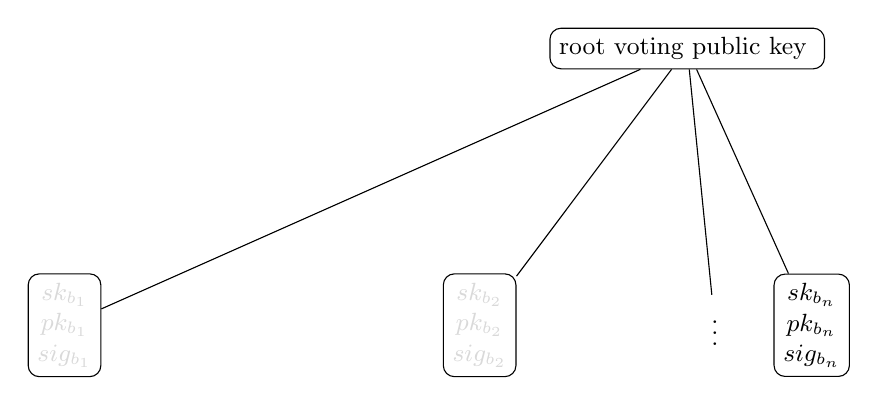
\begin{tikzpicture}[font=\small,every node/.style = {shape=rectangle, rounded corners, draw, align=center}]]
		\tikzset{
			used/.style = { text=gray!30 },
			unused/.style = { text=black },
		}
		\tikzstyle{level 1}=[level distance=10em]
		\tikzstyle{level 2}=[level distance=6em]
		\node { root voting public key }
			child [used, sibling distance=15em] { \key{b_1} }
			child [used, sibling distance=15em] { \key{b_2} }
			child [sibling distance=2em] { node[draw=none] { \vdots } }
			child [sibling distance=3em] { \key{b_n} };
		\end{tikzpicture}
	}{Voting key list}
\end{figure}

The list is completely built before announcing a voting key link transaction.
First, the \emph{root voting key pair} is generated.
The root voting public key is signed with an account's signing public key as part of the voting key link transaction.

Next, epoch-bound keys are generated.
For each key pair, the root key pair signs the epoch-bound public key concatenated with its respective epoch.
After all the epoch-bound keys are generated, the \emph{root voting secret key} is discarded.
In the equations, \emph{i} refers to the respective epoch.
\begin{align*}
	\mathvar{sig}_{b_i} &= \mathfunc{Sign}_{\mathname{root secret key}}(\mathvar{pk}_{b_i} || \mathfunc{IntToBin}(i))
\end{align*}

When signing a voting message for a given epoch, a message signature is created:
\begin{align*}
	\mathvar{sig}_{\mathname{message-i}} &= \mathfunc{Sign}_{\mathvar{sk}_{b_{i}}}(message)
\end{align*}

\subsubsection{Signature}
\index{signature!voting}

The signature for a vote in a given epoch is composed of two pairs:
\begin{itemize}
	\item{$(\mathname{root voting public key}, \mathvar{sig}_{b_i} )$}
	\item{$(\mathvar{pk}_{b_{i}}, \mathvar{sig}_{\mathname{message-i}})$}
\end{itemize}

A \emph{voting key list signature} is considered verified when:
\begin{itemize}
	\item{\emph{root voting public key} is registered to participate in the given epoch.}
	\item{\emph{message} signer key matches epoch-bound key.}
	\item{All component signatures are cryptographically verified.}
\end{itemize}
